\documentclass[%handout,
11pt,a4paper,xcolor={usenames,dvipsnames}]{beamer}
\setbeamertemplate{navigation symbols}{}
\usepackage{lgdv/beamerthemetest}
\usepackage[utf8]{inputenc}
\usepackage{amsmath}
\usepackage{amsfonts}
\usepackage{amssymb}
\usepackage{graphicx}
\usepackage{caption}
\usepackage{subfig}
\usepackage{array}
\usepackage{tabularx}
\usepackage{listings}
\usepackage{multicol}
\usepackage{changepage}

\definecolor{mygreen}{rgb}{0,0.6,0}
\definecolor{mygray}{rgb}{0.5,0.5,0.5}
\definecolor{mymauve}{rgb}{0.58,0,0.82}

\lstset{
	basicstyle=\ttfamily\normalsize,
	language=Python,
	keywordstyle=\color{mygreen},
	showspaces=false,
	showstringspaces=false,
	stringstyle=\color{mymauve},
	commentstyle=\normalfont\color{mygray},
	keepspaces=true,
	columns=fullflexible,
}
\captionsetup[subfloat]{labelformat=empty}
\captionsetup[figure]{labelformat=empty}
\captionsetup[table]{labelformat=empty}


\setlength{\columnsep}{0.1cm}
\setcounter{tocdepth}{2}

%% Hier ändern
\author{Jennifer Kane, Jonas Gröger}
\date{\today}

\begin{document}
    \begin{frame}[plain]
    \title{Informationsvisualisierung}
	\subtitle{Übungspräsentation}
	\titlepage
    \end{frame}
    
       \begin{frame}{6.1 Konzeptionierung einer interaktiven Visualisierung}{Beschreibung des Anwendungsgebiets und der Daten}
        \begin{figure}
    		\centering
    		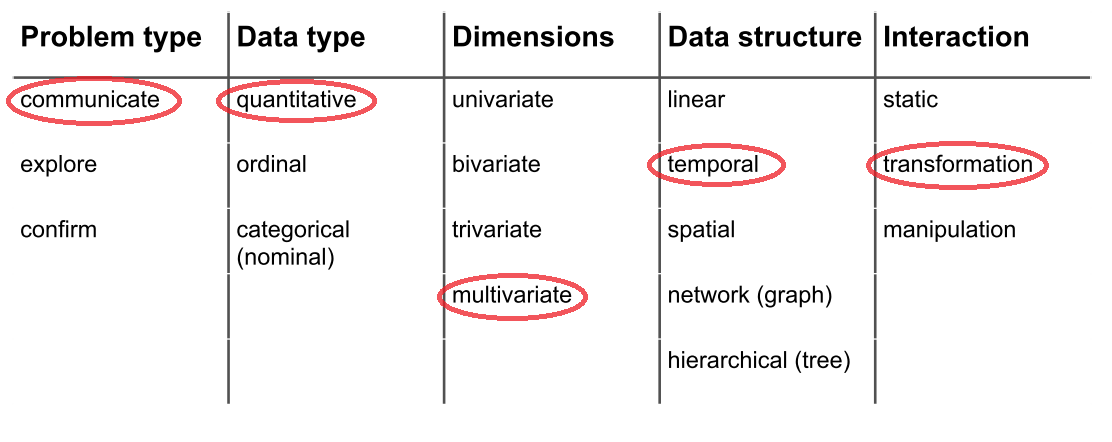
\includegraphics[height=4cm]{includes/datentypen}
		\end{figure}
    \end{frame}

    \begin{frame}{6.1 Konzeptionierung einer interaktiven Visualisierung}{Beschreibung des Anwendungsgebiets und der Daten}
        \begin{itemize}
            \item bestimmte Zeitpunkte hervorgehoben
            \item Vergleich der Zucker-/Koffein-/Alkoholwerte mit empfohlener Maximaldoses
            \item Granularitätsstufen: Tag, Monat, Jahr
        \end{itemize}
    \end{frame}

    \begin{frame}{6.1 Konzeptionierung einer interaktiven Visualisierung}{Zielgruppenanalyse}
        \begin{itemize}
            \item medizinisches Fachpersonal (Ärzte, Psychotherapeuten, ...)
            \item wenig Zeit für einzelnen Patienten $\rightarrow$ Erleichterung durch effiziente Visualisierungen
            \item Visualisierungstechniken: 3D-Abbildungen von Körperteilen, Zeitreihen
        \end{itemize}
    \end{frame}

    \begin{frame}{6.1 Konzeptionierung einer interaktiven Visualisierung}{Zweck der Visualisierung}
        \begin{itemize}
            \item Überblick über den Gesundheitszustand
des Patienten
			\item auf Probleme aufmerksam machen
			\item Detailinformationen zur Getränke- und Inhaltsstoffaufnahme
        \end{itemize}
    \end{frame}

    \begin{frame}{6.1 Konzeptionierung einer interaktiven Visualisierung}{Konzept}
        \begin{itemize}
            \item DEMO
        \end{itemize}
    \end{frame}   
    
    \begin{frame}{Informationsvisualisierung}{Übungspräsentation}
    	Vielen Dank für die Aufmerksamkeit.
    \end{frame}

\end{document}
